\textbf{2-1.}在习题 2-1 图中, 人的质量 $m_{1} = 60 \mathrm{~kg}$ , 底板的质量 $m_{2} = 40 \mathrm{~kg}$ 。人若

想站在底板上静止不动,则必须以多大的力拉住绳子?

\begin{figure}[H]
  \centering
  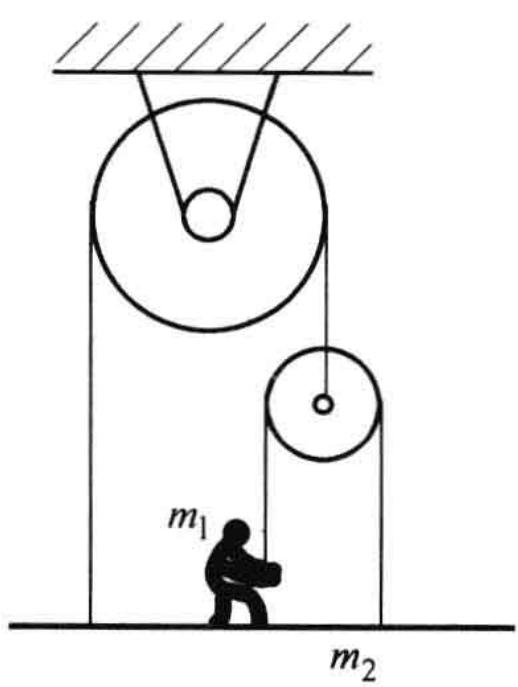
\includegraphics[width=0.2\textwidth]{figures/fig2-1.jpg}
  \end{figure}

\vfill

\textbf{2-2.}一根质量为 $m_{0}$ 的均质绳子, 两端固定在同一高度的两个钉子上, 在其中点挂一质量为 $m$ 的物体。设 $\alpha, \beta$ 分别为在绳子中点和端点处绳子的切线方向与竖直方向的夹角, 如习题 2- 2 图所示。求 $\frac{\tan \alpha}{\tan \beta}$ 与 $m_{0}, m$ 的关系。

\begin{figure}[H]
  \centering
  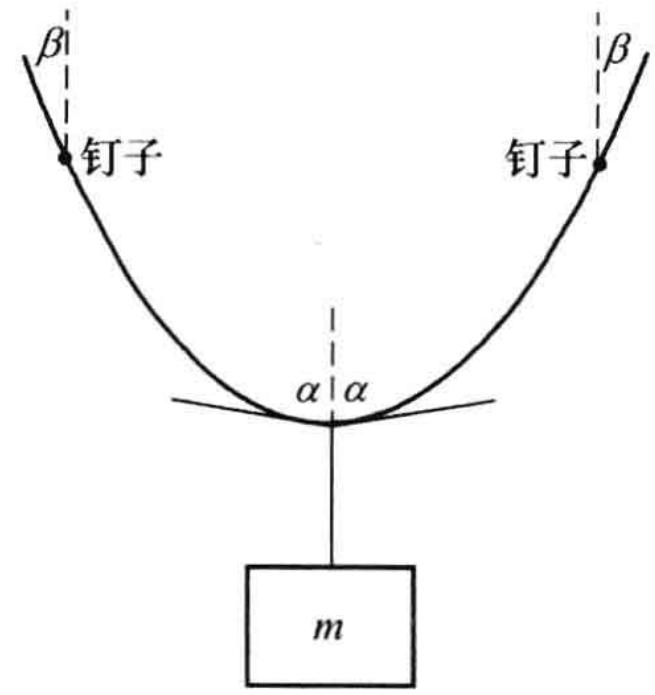
\includegraphics[width=0.25\textwidth]{figures/fig2-2.jpg}
  \end{figure}

\vfill
\newpage

\textbf{2-3.}如习题 2-3 图(a)所示,一长为 $l$ 、质量为 $m$ 的均匀链条套在一表面光滑、顶角为 $\alpha$ 的圆锥上,当链条在圆锥面上静止时,求链中的张力。

\begin{figure}[H]
  \centering
  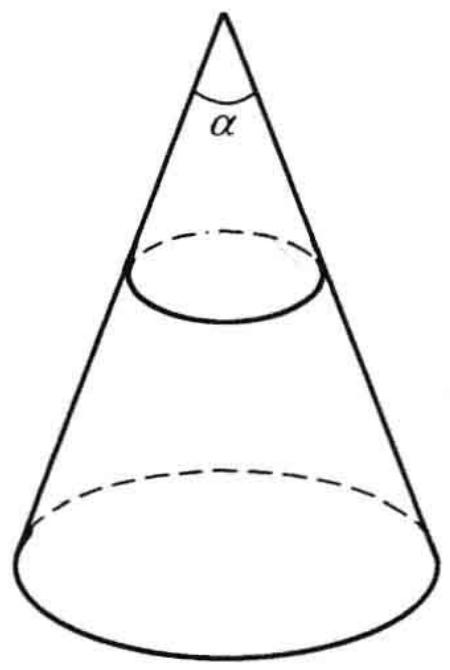
\includegraphics[width=0.2\textwidth]{figures/fig2-3_a.jpg}
  \end{figure}

\vfill

\textbf{2-4.}一条绳索的一端系到停泊在河中的小船上,另一端由站在岸上的人拿着。人正欲收绳把船拉往岸边时,突然刮起了大风,风把船吹向河心。为了不让风把船吹走,人把绳索在岸边的固定圆柱上缠绕若干圈后再拉住绳索。若由于大风使船与圆柱间的绳索中的张力变为 $50000 \mathrm{~N}$ , 而人拉绳的最大力为 $500 \mathrm{~N}$ 。已知绳索与圆柱之间的摩擦因数为 0.32 ,问绳索至少在圆柱上绕几圈,船才不会被吹走?

\begin{figure}[H]
  \centering
  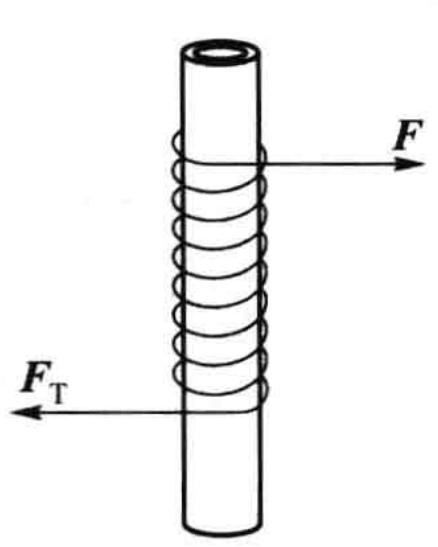
\includegraphics[width=0.2\textwidth]{figures/fig2-4_a.jpg}
  \end{figure}

\vfill
\newpage

\textbf{2-5.}在习题 2-5 图中, 物体 A 和 B 的质量分别为 $m_{\mathrm{A}}$ 和 $m_{\mathrm{B}}$ , 用跨过定滑轮

的细线相连,静止地叠放在倾角为 $\theta$ 的斜面上,各接触面的静摩擦因数为 $\mu$ ,现有一平行于斜面的力 F 作用在物体 A 上,问 F 至少为多大才能使两物体运动?

\begin{figure}[H]
  \centering
  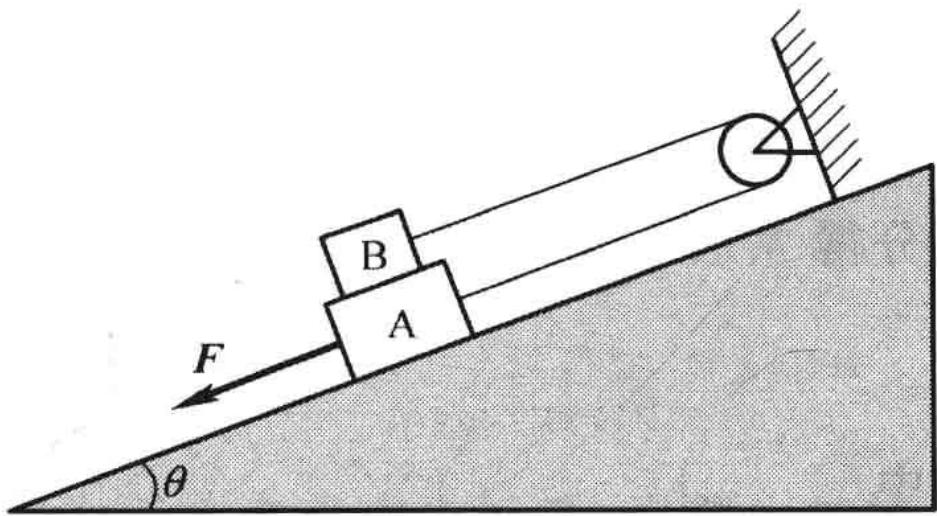
\includegraphics[width=0.3\textwidth]{figures/fig2-5.jpg}
  \end{figure}

\vfill

\textbf{2-6.}质量为 $m_{1}$ 的气球以加速度 $a$ 匀加速上升, 突然一只质量为 $m_{2}$ 的小鸟飞到气球上, 并停留在气球上。若气球仍能向上加速, 求气球的加速度减少了多少?

\vfill
\newpage

\textbf{2-7.}一质量为 $m$ 的汽艇在湖水中以速率 $v_{0}$ 直线运动, 当关闭发动机后, 受水的阻力为 $F_{\mathrm{f}} = -k v$ , 求速度、位移随时间的变化关系。

\vfill

\textbf{2-8.}质量分别为 $m_{1}$ 和 $m_{2}(m_{2} > m_{1})$ 的两个人, 分别拉住跨在定滑轮 (忽略质量) 上的轻绳两边往上爬。开始时两人至定滑轮的距离都是 $h$ 。试证明: 质量为 $m_{1}$ 的人经过时间 $t$ 爬到滑轮处时, 质量为 $m_{2}$ 的人与滑轮的距离为 $\frac{m_{2} - m_{1}}{m_{2}}\left(h + \frac{1}{2}gt^{2}\right)$ 。

\begin{figure}[H]
  \centering
  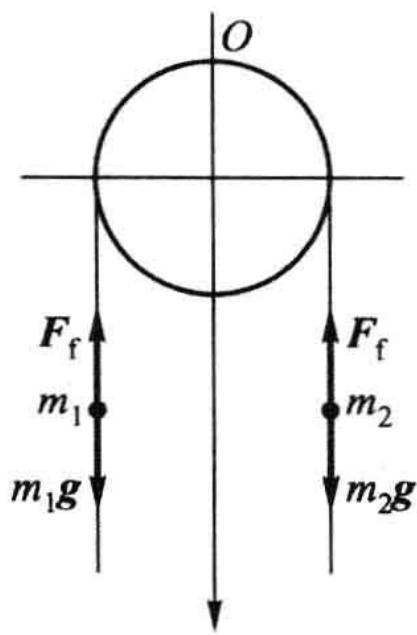
\includegraphics[width=0.2\textwidth]{figures/fig2-8.jpg}
  \end{figure}

\vfill
\newpage

\textbf{2-9.}一物体以 $v_{0}$ 的初速度做竖直上抛运动, 若受到的阻力 $F_{\mathrm{f}}$ 与其速度的二次方 $v^{2}$ 成正比, 大小可表示为 $F_{\mathrm{f}} = m g k^{2} v^{2}$ , 其中 $m$ 为物体的质量, $k$ 为常量。试证明此物体回到上抛点时的速度为 $v_{1} = \sqrt{\frac{v_{0}^{2}}{1 + (k v_{0})^{2}}}$ 。

\vfill

\textbf{2-10.}一半顶角为 $\alpha$ 的倒立圆锥面的内表面光滑, 内表面上一质点绕对称轴做半径为 $r$ 的匀速圆周运动。求质点的速率。

\vfill
\newpage

\textbf{2-11.}如习题 2-11 图所示, 两个物体的质量分别为 $m_{1} = 15 \mathrm{~kg}, m_{2} = 20 \mathrm{~kg}$ , 作用在物体 $m_{1}$ 上的水平力 $F = 280 \mathrm{~N}$ 。设所有接触面都光滑。试求:

(1) $m_{1}$ 的加速度的大小和方向；

(2) $m_{2}$ 的加速度的大小和方向；

(3) 两物体间的相互作用力。

\begin{figure}[H]
  \centering
  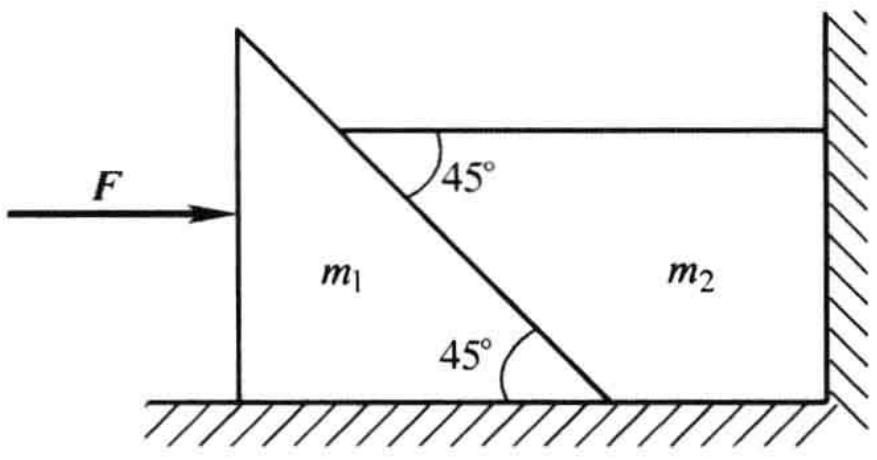
\includegraphics[width=0.3\textwidth]{figures/fig2-11.jpg}
  \end{figure}

\vfill

\textbf{2-12.}从地面以相对地面成 $\theta_0$ 仰角、 $v_0$ 的速度发射一炮弹, 炮弹在运动过程中始终受到与速度成正比的阻力 $F_{\mathrm{f}} = kv (k$ 为常量) 作用, 求炮弹的运动轨迹方程。

\vfill
\newpage



\textbf{2-13.}如习题 2-13 图所示的系统, 系统中人的质量 $m_{1} = 60 \mathrm{~kg}$ , 人所站着的底板质量 $m_{2} = 20 \mathrm{~kg}$ , 绳子和滑轮质量均可忽略不计。人要用多大的力拉住绳子, 才能保持自己和底板静止不动?

\begin{figure}[H]
  \centering
  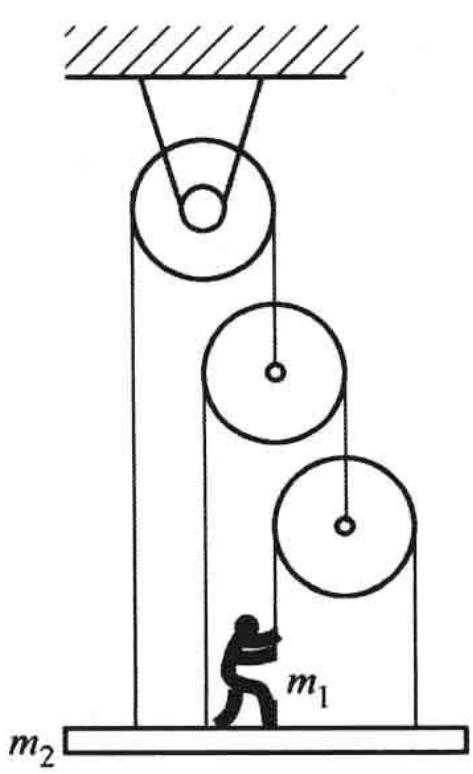
\includegraphics[width=0.2\textwidth]{figures/fig2-13_2.jpg}
  \end{figure}

\vfill

\textbf{2-14.}质量为 $m_{1}$ 和 $m_{2}$ 的两物体, 在水平力 $F$ 的作用下紧靠在墙上, 如习题 2-14 图所示。为使两物块均不掉下, 试问在以下两种情况下, $F$ 至少应为多大?

(1) 各接触面间的静摩擦因数均为 $\mu$ 时；

(2) $m_{1}, m_{2}$ 之间的静摩擦因数为 $\mu_{1}, m_{2}$ 与墙面间的静摩擦因数为 $\mu_{2}$ 时。

\begin{figure}[H]
  \centering
  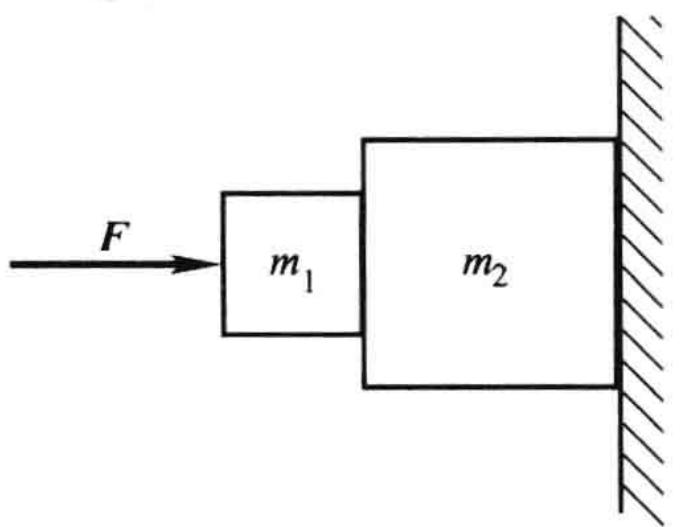
\includegraphics[width=0.3\textwidth]{figures/fig2-14.jpg}
  \end{figure}

\vfill
\newpage

\textbf{2-15.}一个三棱柱固定在桌面上, 形成两个倾角分别为 $\alpha$ 和 $\beta$ 的斜面, 一细绳跨过顶角处的滑轮与质量分别为 $m_{1}$ 和 $m_{2}$ 的两物体相连, 如习题 2-15 图所示。已知物体与斜面间的静摩擦因数均为 $\mu$ , 求两物体在斜面上保持静止的条件。

\begin{figure}[H]
  \centering
  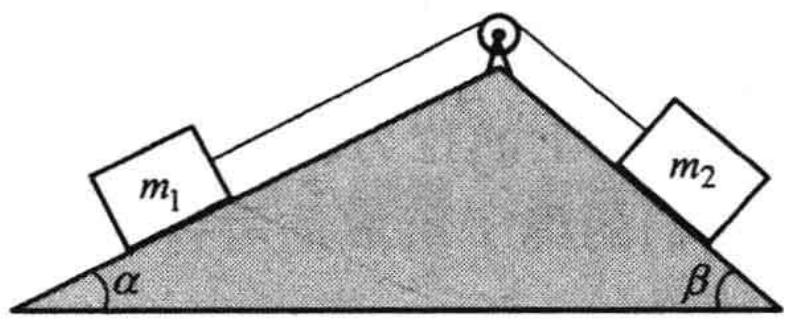
\includegraphics[width=0.3\textwidth]{figures/fig2-15.jpg}
  \end{figure}

\vfill

\textbf{2-16.}三块质量均为 $m$ 的相同物块叠放在水平面上, 如习题 2-16 图所示。已知各接触面的摩擦因数均为$\mu$。

(1) 现有一水平力 F 作用在最底下的物块上, 使之从上面两物块下抽出, 则 F 至少为多大?

(2) 若水平力 $F$ 作用在中间的物块上,使它从上、下两物块中抽出, 则 $F$ 至少为多大?

\begin{figure}[H]
  \centering
  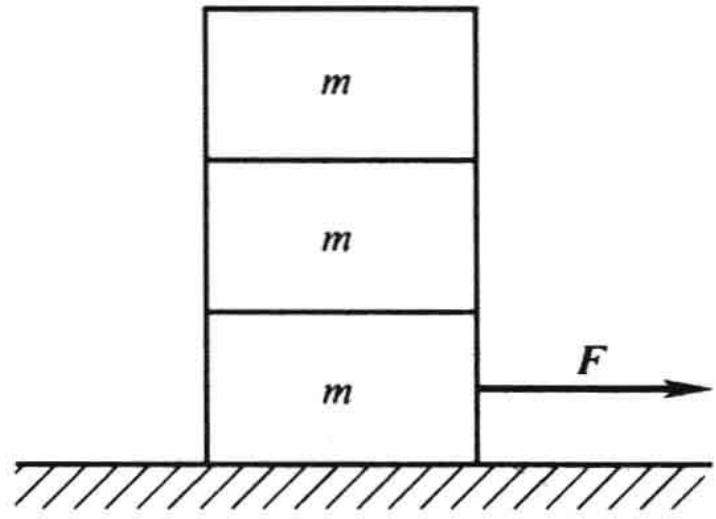
\includegraphics[width=0.3\textwidth]{figures/fig2-16.jpg}
  \end{figure}

\vfill
\newpage

\textbf{2-17.}如习题 2-17 图所示, 质量分别为 $m_{1}$ 和 $m_{2}$ 的两物体用一细绳相连, 细绳跨过装在另一质量为 $m_{0}$ 的大物体上的定滑轮, 使 $m_{1}$ 和 $m_{2}$ 分别与 $m_{0}$ 上的水平面和倾角为 $\theta$ 的斜面接触, 而整个系统放在水平地面上。设 $m_{1}, m_{2}$ 与 $m_{0}$ 间的接触面都光滑。试问, 若要 $m_{0}$ 保持静止, 则 $m_{0}$ 与水平地面之间的摩擦因数至少为多大?

\begin{figure}[H]
  \centering
  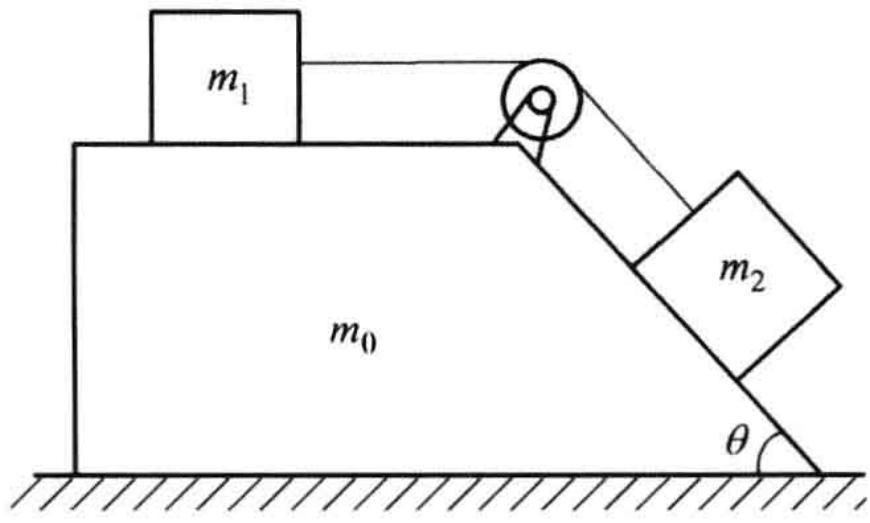
\includegraphics[width=0.3\textwidth]{figures/fig2-17.jpg}
  \end{figure}

\vfill

\textbf{2-18.}一条质量为 $m$ 的均匀绳索悬结于两座高度相等的山顶之间, 绳索在悬结处与竖直方向的夹角均为 $\theta$ , 如习题 2-18 图所示。试求:

(1) 两山顶各自受到的绳索的作用力的大小;

(2) 绳索中点处的张力。

\begin{figure}[H]
  \centering
  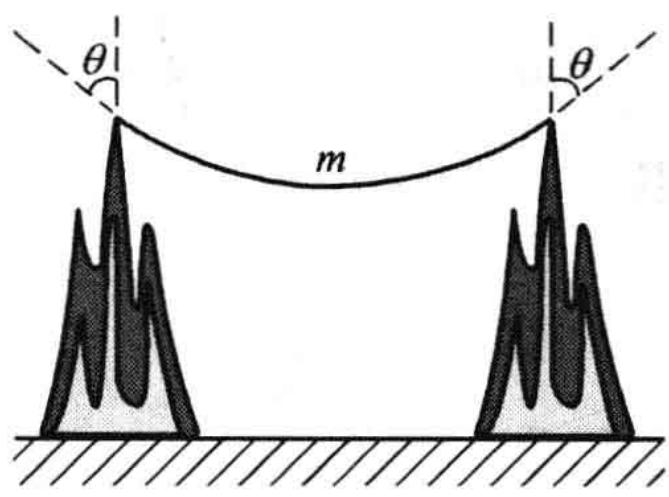
\includegraphics[width=0.3\textwidth]{figures/fig2-18_x.jpg}
  \end{figure}

\vfill
\newpage

\textbf{2-19.}一个质量为 $m$ 的物体通过一根质量可以不计的绳子绕水平棒 $1 \frac{1}{4}$ 周后于另一端加一水平力 $F$ , 如习题 2-19 图 (a) 所示。若绳子和棒之间的摩擦因数为 $\mu$ , 要使物体保持静止状态, 应施加多大的水平拉力?

\begin{figure}[H]
  \centering
  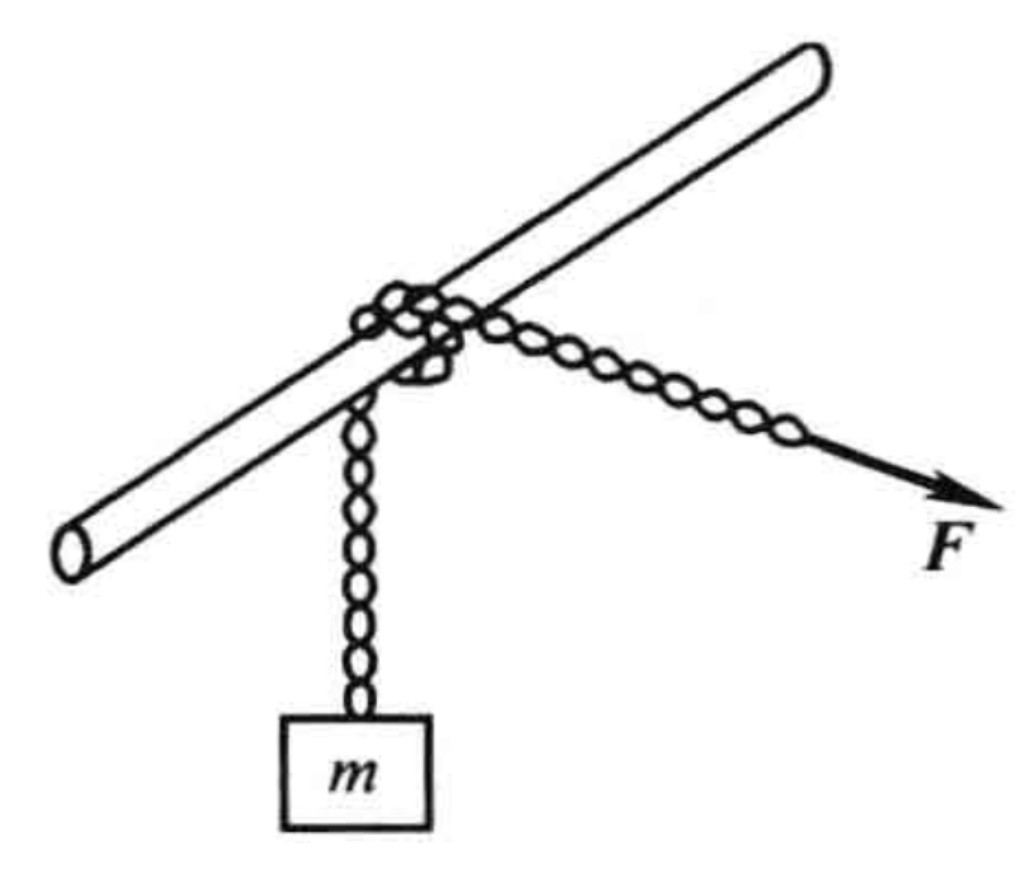
\includegraphics[width=0.3\textwidth]{figures/fig2-19_a.jpg}
  \end{figure}


\vfill

\textbf{2-20.}两物体的质量分别为 $m_0$ 和 $m$ , 用一根质量可以忽略的细绳相连, 细绳跨过装置在桌面上的定滑轮, 使物体 $m_0$ 放在光滑的桌面上, 而物体 $m$ 悬在桌边, 如习题 2-20 图所示。求物体 $m_0$ 运动的加速度。若将物体 $m$ 拿去, 而用大小为 $mg$ 的力向下拉绳, 则物体 $m_0$ 的加速度是否发生变化? 略去滑轮的质量和滑轮轴承处的摩擦力, 且细绳不能伸长。

\begin{figure}[H]
  \centering
  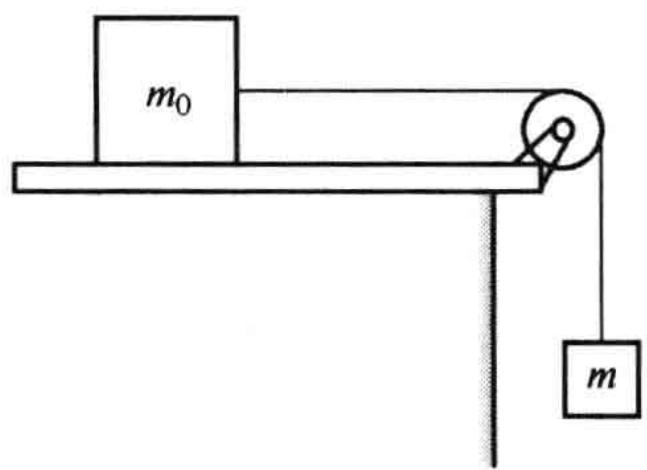
\includegraphics[width=0.3\textwidth]{figures/fig2-20.jpg}
  \end{figure}

\vfill
\newpage

\textbf{2-21.}一质量为 $50 \mathrm{~kg}$ 的人站在电梯里的台秤上, 求:

(1) 当电梯以 $4.9 \mathrm{~m} / \mathrm{s}$ 的速度匀速上升或下降时, 台秤读数各是多少?

(2) 当电梯以 $4.9 \mathrm{~m} / \mathrm{s}^{2}$ 的加速度上升或下降时, 台秤读数又各是多少?

\vfill

\textbf{2-22.}一飞机在竖直平面内以 $540 \mathrm{~km} / \mathrm{h}$ 的速度沿一圆周飞行。为使在飞机飞行过程中,驾驶员与座椅之间的相互作用力不大于驾驶员重力的 8 倍,试求此圆周的最小半径。

\vfill
\newpage

\textbf{2-23.}一质量为 $m$ 的物体静止于倾角为 $\theta$ 的固定斜面上, 如习题 2-23 图所示。已知物体与斜面间的静摩擦因数为 $\mu$ , 试问, 至少要用多大的力作用在物体上, 才能使它运动? 并指出该力的方向。

\begin{figure}[H]
  \centering
  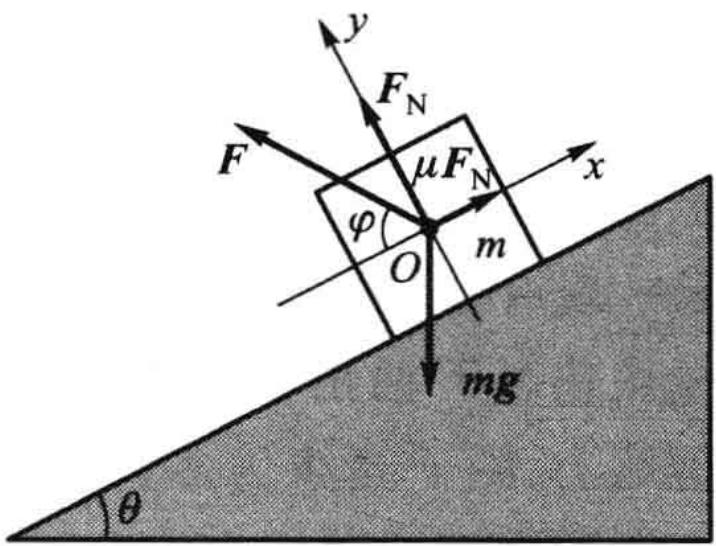
\includegraphics[width=0.25\textwidth]{figures/fig2-23.jpg}
  \end{figure}

\vfill

\textbf{2-24.}两个质量均为 $m$ 的质点 $A$ 和 $B$ 连在一个劲度系数为 $k$ 的弹簧的两端。开始两质点静止在光滑的水平面上,弹簧处于原长,然后沿 AB 方向给 B 以恒力 ka。求两质点的运动学方程。

\vfill
\newpage

\textbf{2-25.}质量为 $m_{0}$ 的木板静置在水平桌面上, 其一端与桌面对齐, 木板上放

一质量为 m 的小花瓶, 花瓶与板左端相距为 l, 桌面长为 L, 如习题 2-25 图所示。现有一水平恒力 F 作用于板上, 将板从花瓶下抽出。为使花瓶不至于掉落地上, 则 F 至少为多大? 设各接触面之间的摩擦因数均为 $\mu$ 。

\begin{figure}[H]
  \centering
  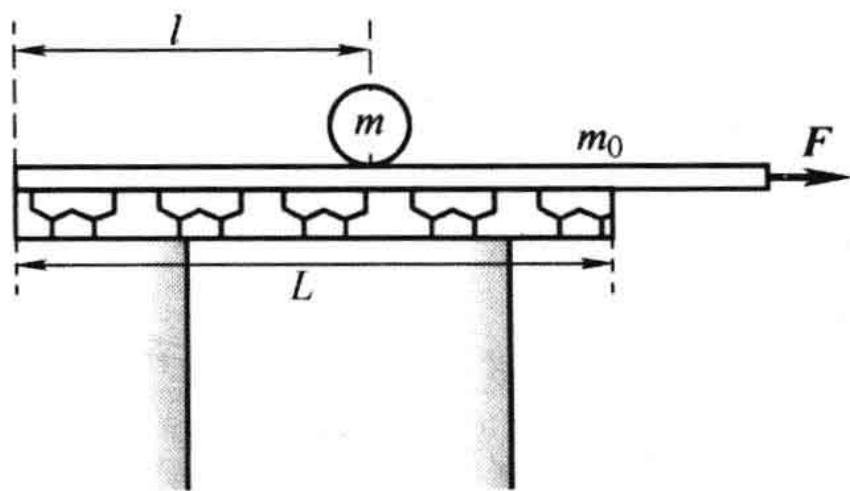
\includegraphics[width=0.3\textwidth]{figures/fig2-25.jpg}
  \end{figure}

\vfill

\textbf{2-26.}如习题 2-26 图所示, 质量分别为 $m_{1}$ 和 $m_{2} (m_{1} > m_{2})$ 的两物体叠放在水平桌面上, 另一质量为 $m_{3}$ 的物体通过细绳和滑轮组与 $m_{1}, m_{2}$ 相连并悬在桌边。

(1) 若 $m_{1}$ 与 $m_{2}$ 之间的摩擦因数为 $\mu$ ，而 $m_{1}$ 与桌面之间无摩擦力，求运动时， $m_{1}$ 与 $m_{2}$ 之间无相对滑动的条件；

(2) 若各接触面之间的摩擦因数均为 $\mu$ , 求 $m_{2}$ 与 $m_{3}$ 运动, 而 $m_{1}$ 保持静止的条件。

\begin{figure}[H]
  \centering
  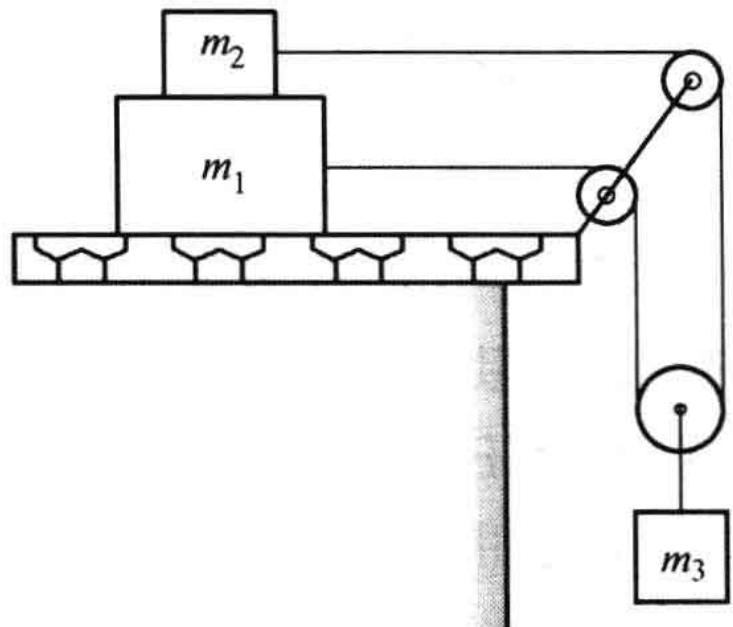
\includegraphics[width=0.25\textwidth]{figures/fig2-26.jpg}
  \end{figure}

\vfill
\newpage

\textbf{2-27.}空中有许多大小不等的雨滴(可看成圆球形)由静止开始下落。若受到的空气阻力 $F_{\mathrm{f}}$ 与其速度 $\nu$ 的一次方成正比, 即 $F_{\mathrm{f}} = -k\nu$ , 其中 $k$ 为常量。

(1) 求任一时刻 t 雨滴的速度 $v(t)$ ;

(2) 证明雨滴的速度最终将趋于一极限值 $v_{f}$ (称为终极速度), 并求出此 $v_{f}$ ;

(3) 若常量 $k$ 正比于各雨滴的大圆面积, 即 $k \propto \pi r^{2}$ ( $r$ 为雨滴的半径), 试问: 大、小雨滴中哪种雨滴获得的终极速度较大?

\vfill

\textbf{2-28.}一子弹以 $v_{0}$ 的初速度和 $\theta$ 仰角自地面射出, 子弹在飞行时受到的空气阻力为其速度的 $km$ 倍 ( $m$ 为子弹的质量, $k$ 为常量)。试求子弹的速度与水平线成 $45^{\circ}$ 角时, 子弹与发射点之间的水平距离 $s$ 。

\begin{figure}[H]
  \centering
  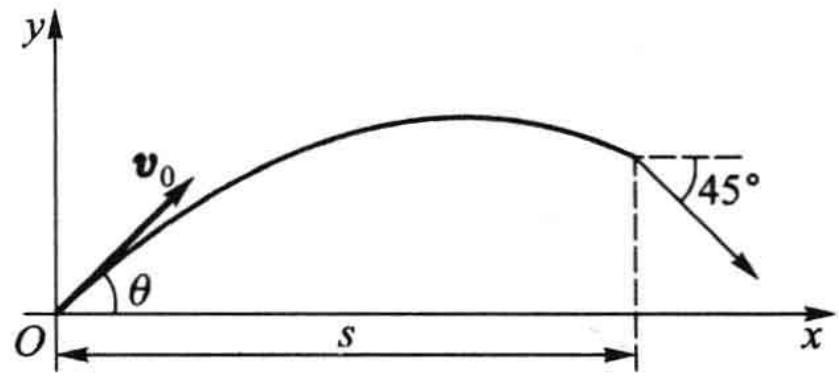
\includegraphics[width=0.3\textwidth]{figures/fig2-28.jpg}
\end{figure}

\vfill
\newpage